\documentclass{article}
\usepackage{amsmath,amssymb,amsthm, graphicx}
\usepackage{mathpazo}
\author{Alexandre Vassalotti \quad \'{E}ric Renaud-Houde}
\title{COMP 558: Final Project Report \\
  \large \textbf{Surface reconstruction using the level set method}
}
\date{27 April 2012}

\begin{document}
\maketitle
\section{Introduction}
Modelling surfaces from unorganized set of points, or point clouds, is a long
standing problem in the computer vision community. Indeed, problem is known to
be very challenging in three and higher dimensions. Furthermore, the problem
is ill-posed which means there is not a unique solution. When the point cloud
is dense enough and the topology of the surface is not complicated, a simple
solution could be to perform a triangulation of points. However, even in this
context ambiguities can arises and lead to non desirable surface
reconstructions.

A desirable reconstruction method should be able to deal with irregularities
caused by noise and non-uniformity of the data collected. A method should also
be able to deal with complex surface topologies as well. In addition, the
reconstructed surface should be representative of the point could data.



\section{Framework}

\paragraph{Discretization}

Given that the surface motion equation for $\phi$ is defined as a partial
differential equation, we can solve it using iterative schemes for PDEs. As most
differential equations which might appear fairly innocuous at first, solving
them numerically can be quite challenging.

Given an initial value $\phi_0$, our first intution might be to apply the
first-order Euler method as follows:
\begin{align}
  \frac{\partial \phi}{\partial t} + F \|\nabla \phi\| &= 0 \\
  \frac{\phi^{t+1} - \phi^{t}}{\Delta t} &=  -F \|\nabla \phi\| \\
  \phi^{t+1} &= \phi^{t} - \Delta t \; F \|\nabla \phi\| 
\end{align}

However, not only does the Euler method often suffers from stability problems,
it is used in the context of \textit{ordinary differential equations}, not PDEs.
In that case, a different numerical procedure is needed. 

\subparagraph{Upwind Scheme}
One approach for discretizing PDEs, originally defined by Couran, Isaacson and
Rees \cite{courant1952solution} is called the upwind scheme. Instead of using
central differences for computing the partial derivatives, it uses both a
forward or a backward difference:

\begin{align}
    \frac{\partial \phi}{\partial x}^{-} &= \phi^{-}_x = \frac{\phi_i -
    \phi_{i-1}}{ \Delta x} = \phi_i - \phi_{i-1} \\
    \frac{\partial \phi}{\partial x}^{+} &= \phi^{+}_x = \frac{\phi^{i+1}_x -
    \phi^i_x}{ \Delta x} = \phi^{i+1}_x - \phi^i_x  
\end{align} since $ \Delta x = 1 $ in our grid. The same applies for other axes
$y$ and $z$.

\begin{figure}[htb]
  \centering
  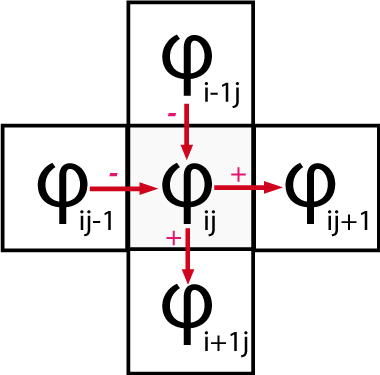
\includegraphics[width=0.45\textwidth]{img/upwind_grid.png}
  \caption{Illustration of the forward and backward differences over a 2d grid.}    
\end{figure}


Later used by Sethian\cite{sethian1999level} \cite{sethian1999advancing} for
the initial value formulation, he defines the classical level set method as
follows (let $ p = \phi_{ijk}$):

\[
p^{n+1} = p^{n} - \Delta t [ \max(F_{ijk}, 0) \| \nabla p \|^{+} + \min(F_{ijk}, 0)
\| \nabla p \|^{-} ]
\]
where:
\begin{align}
    \| \nabla p \|^{+} & = 
    \begin{bmatrix}
        \max(p^{-}_x, 0)^2 + \min(p^{+}_x, 0)^2 + \\
        \max(p^{-}_y, 0)^2 + \min(p^{+}_y, 0)^2 + \\
        \max(p^{-}_z, 0)^2 + \min(p^{+}_z, 0)^2
    \end{bmatrix}^{1/2}  \\
    \| \nabla p \|^{-} & = 
    \begin{bmatrix}
        \max(p^{+}_x, 0)^2 + \min(p^{-}_x, 0)^2 + \\
        \max(p^{+}_y, 0)^2 + \min(p^{-}_y, 0)^2 + \\
        \max(p^{+}_z, 0)^2 + \min(p^{-}_z, 0)^2
    \end{bmatrix}^{1/2} 
\end{align}

Rewriting this equation in terms of the entire grid matrices, and defining
$\odot$ as element-wise matrix mutiplication, we have the following formulation
which updates our entire grid for $\phi$:
\[
\phi^{n+1} = \phi^{n} - \Delta t [ \max(F, 0) \odot \| \nabla \phi \|^{+} +
\min(F, 0) \odot \| \nabla \phi \|^{-} ]
\]

As opposed to computing the magnitude of the gradient using the central
differences functions, the evolution of $\phi$ under the upwind scheme is much
more stable. Note that there are higher-order schemes listed in
\cite{sethian1999level} if more stability is required.

\begin{figure}[htb]
  \centering
  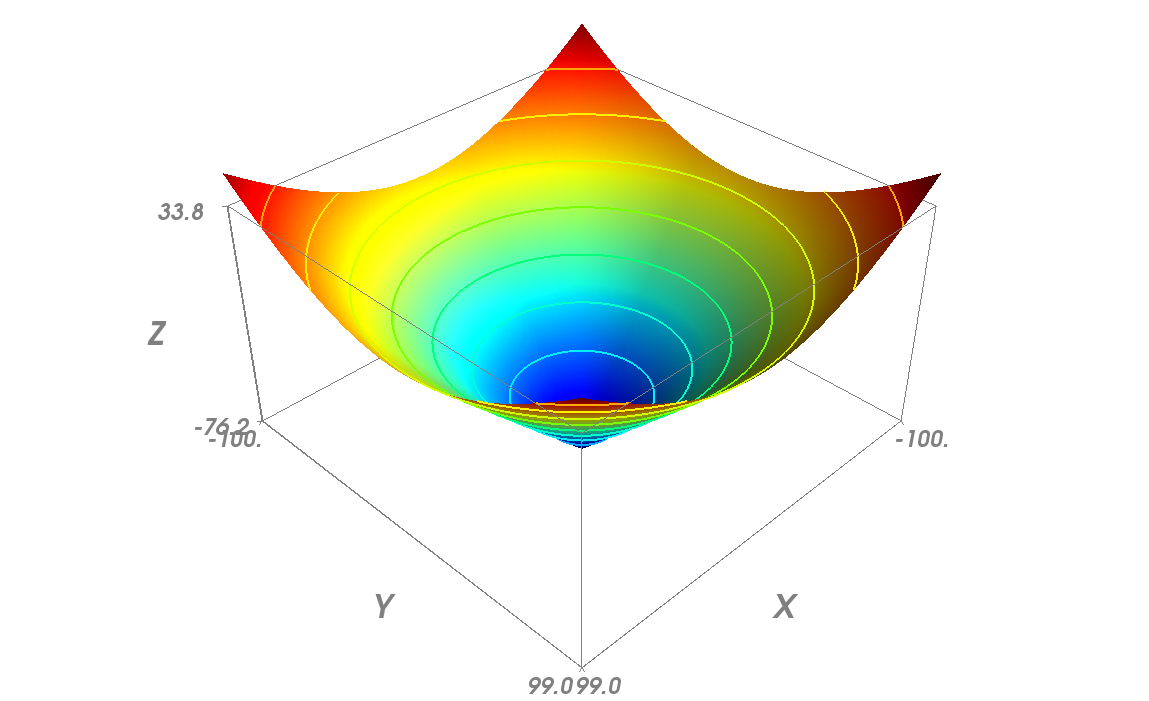
\includegraphics[width=0.8\textwidth]{img/up01.png}
  \caption{Initial hypersurface $\phi$ defined as a signed distance function
  (for a level set in 2d).}    
\end{figure}

\begin{figure}[htb]
  \centering
  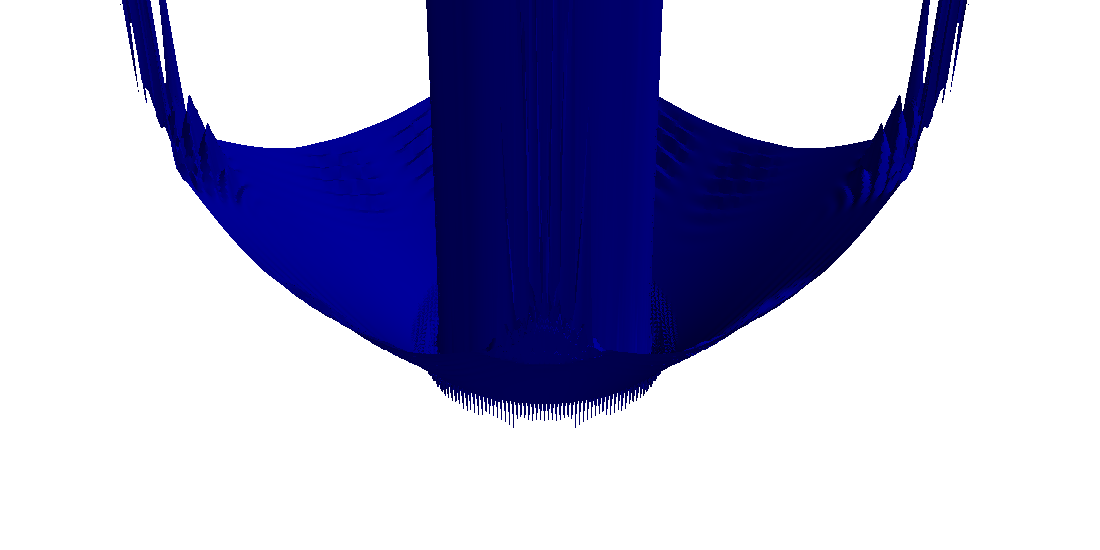
\includegraphics[width=0.8\textwidth]{img/up03.png}
  \caption{Result of 140 iterations using $\Delta t = 0.5$ and a constant force of 1
  using the central differences approximations. The resulting hypersurface has
  exploded in the center and near
  the borders.}    
\end{figure}

\begin{figure}[htb]
  \centering
  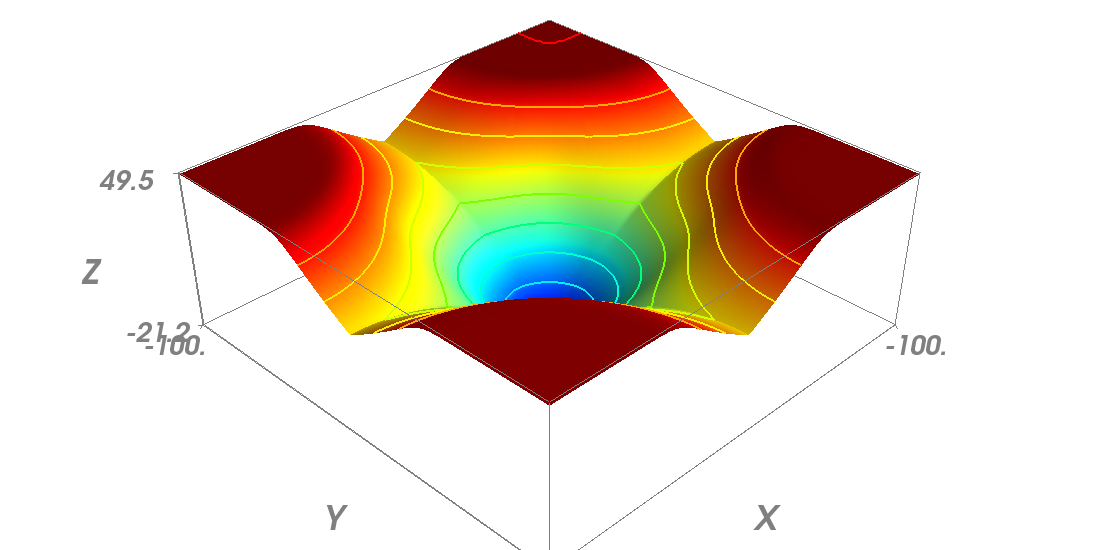
\includegraphics[width=0.8\textwidth]{img/up02.png}
  \caption{Result of 140 iterations using $ \Delta t = 0.5$ and a constant force of 1
  using the upwind scheme. The hypersurface evolution is perfectly stable. It
  ultimately flattens out and remain so.}    
\end{figure}

\subparagraph{Implementation}
To implement the upwind scheme for the entire grid update, a few strategies can
be used. In the contex of matlab or numpy, it is recommended to compute forward
and backward differences using entire rows. Also note that only one matrix is
needed because the squared differences can be added on top of each other.
Furthermore for the edges of the grid, the inward row/column should be used in
replacement if the difference exceeds the matrix.

\bibliographystyle{amsplain}
\bibliography{vision}

\end{document}
